\chapter{Reinforcement Learning For SQL Query Optimization}
\chaptermark{Query Optimization}
Joins are a ubiquitous primitive in data analytics. 
The rise of new tools, such as Tableau, that automatically generate queries has led to renewed interest in efficiently executing SQL queries with several hundred joined relations.
Since most relational database management systems support only dyadic join operators (joining two tables) as primitive operations, a query optimizer must choose the ``best'' sequence of two-way joins to achieve the k-way join of tables requested by a query. 

\section{Problem Setup}
The problem of optimally nesting dyadic joins is, of course, combinatorial and is known to be NP-Hard.
To make matters worse, the problem is also known to be practically challenging since a poor solution can execute several orders of magnitude slower than an optimal one.
Thus, many database systems favor ``exact'' solutions when the number of relations are small but switch to approximations after a certain point.
For example, PostgreSQL uses dynamic programming when the query has less than 12 relations and
then switches to a genetic algorithm for larger queries. 
Similarly, IBM DB2 uses dynamic programming and switches to a greedy strategy when the number of relations grows.

Traditionally, exact optimization is addressed with a form of sequential dynamic programming. 
The optimizer incrementally builds optimal joins on subsets of relations and memoizes the optimal join strategy as well as the cost-to-go based on an internal cost model. 
This dynamic programming algorithm still enumerates all possible join sequences but shares computation where possible.
Natually, this enumeration process is sensitive when the underlying cost models in the RDBMS are inaccurate.
Care has to be taken to avoid enumerating plans that are risky, or high variance, if table sizes or system parameters are not known exactly.
Some work has considered incorporating feedback to the cost model after execution to improve the model for future optimization instances. 

As it stands there are three challenges that modern join optimizers try to simultaneously address: (1) pruning a large space of possible plans, (2) hedging against uncertainty, and (3) feedback from query evaluation. For each of these three problems, the community has proposed numerous algorithms, approximations, and heuristics to address them. Often the dominant techniques are sensitive to both the particular workload and the data. The engineering complexity of implementing robust solutions to all of these challenges can be very significant, and commerical solutions are often incomplete---where some level of query engineering (by creating views and hints) from the developer is needed.

Recent advances in Artificial Intelligence may provide an unexpected perspective on this impasse.
The emergence of deep reinforcement learning, e.g., AlphaGo, has presented a pragmatic solution to many hard Markov Decision Processes (MDPs).
In an MDP, there is a decision making agent who makes a sequence of decisions to effect change on a system that processes these decisions and updates the system's internal state (potentially non-deterministically). 
MDPs are Markovian in the sense that the system's current state and the agent's decision completely determines any future evolution.
The solution to an MDP is a decision to make at every possible state.
We show that the join optimization can be posed as an MDP where the state is the join graph and decisions are edge contractions on this graph.

Given this formulation, the Deep Q Network (DQN) algorithm can be applied, and in essence, this formulation gives us an approximate dynamic programming algorithm.
Instead of exactly memoizing subplans in a table with cost-to-go estimates as in dynamic programming, DQN represents this table with a neural network of a fixed size.
This allows the algorithm to ``estimate'' the cost-to-go of subplans even if they have not been previously enumerated.

This learning based approach gives us flexibility in designing new intelligent enumeration strategies by manipulating how the neural network is trained and how it represents the subplans.
For example, the neural network allows us to efficiently share query processing information across planning instances with the neural network parameters and learn from previously executed queries.
The consequence is enumeration strategies tuned to the specific workload and data.
We can also vary the features used to represent the subplans, to allow the network to capture different properties like interesting orders and physical operator selection.
We can also train the neural network with observations of actual query execution times and make through repeated executions make it robust to uncertainty.

In short, Deep RL provides a new algorithmic framework for thinking about join enumeration. 
We can architect an entire query processing stack around this Deep RL framework.
In this paper, we explore this architecture and evaluate in what situations its behavior is more desirable (either in terms of cost or planning time) compared to classical approaches.
Our system is built on Apache Calcite and integrates with Apache Spark, Postgres SQL, and an internal join planning simulator.
We present results on a variety of experimental workloads and datasets.

\subsection*{Problem Statement}
Consider the following query model.
Let $\{R_1,...,R_k\}$ define a set of relations, and let $\mathcal{R} = R_1 \times ... \times R_k$ denote the cartesian product.
We define an inner join query $q$ as a subset of $q \subseteq \mathcal{R}$ as defined by a conjunctive predicate $\rho_1 \wedge ... \wedge \rho_j$ where each expression $\rho$ is binary boolean function of the attributes of two relations in the set $\rho = f(R_i.a, R_j.b)$.
Extending our work to consider left and right outer joins is very straight-forward but we will defer that to that to future work.

\subsubsection{Example}
Suppose, we have a database of three relations denoting employee salries:
\[
\text{Emp}(id, name, rank)
\]
\[
\text{Pos}(rank, title, code)
\]
\[
\text{Sal}(code, amount)
\]
Consider the following join query:
\begin{lstlisting}
SELECT *
 FROM Emp, Pos, Sal
 WHERE Emp.rank = Pos.rank AND
 Pos.code = Sal.code
\end{lstlisting}
In this schema, $\mathcal{R}$ denotes the set of tuples $\{(e \in Emp, p \in Pos, s \in Sal)\}$. There are two predicates $\rho_1 = Emp.rank = Pos.rank$ and $\rho_2 = Pos.code = Sal.code$, combined with a conjunction. 

\subsubsection{Join Optimization}
Outside of the academic literature, most commercial query processing engines can only execute ``dyadic'' joins, that is, joins between two relations. In the above query, one has several possible options on how to execute that query. For example, one could execute the query as $Emp \bowtie (Sal \bowtie Pos)$. Or, one could execute the query as $Sal \bowtie (Emp \bowtie Pos)$. Enumerating all such executions grows combinatorially even if the join $\bowtie$ is symmetric and commutative.
We assume that the join operation is commutative, left associative, and right associative.

\subsubsection{Query Graph Model}
Enumerating the set of all possible dyadic join plans can be elegantly expressed as operations on a graph.

\begin{definition}[Query Graph]
Let $G$ define an undirected graph called the \emph{query graph}, where each relation $R$ is a vertex and each $\rho$ defines an edge between vertices. The number of connected components of $G$ are denoted by $\kappa_G$.
\end{definition}

Each possible dyadic join is equivalent to a combinatorial operation called a graph contraction.

\begin{definition}[Contraction]
Let $G = (V,E)$ be a query graph with V defining the set of relations and E defining the edges from the join predicates. A contraction $c$ is a function of the graph parametrized by a tuple of vertices $c=(v_i, v_j)$. Applying $c$ to the graph $G$ defines a new graph with the following properties: (1) $v_i$ and $v_j$ are removed from $V$, (2) a new vertex $v_{ij}$ is added to $V$, and (3) the edges of $v_{ij}$ are the union of the edges incident to $v_i$ and $v_j$. 
\end{definition}

Note that each contraction reduces the number of vertices by $1$. And, that every feasible dyadic join plan can be described as a sequence of such contractions $c_1 \circ c_2 ...\circ c_{T}$ until $|V| = \kappa_G$. The number of possible contraction sequences is upper bounded by $\mathcal{O}(|V|^{|V|})$. 

The sequence of contractions exactly corresponds to a dyadic join plan. Going back to our running example, suppose we start with a query graph consisting of the vertices $(Emp, Pos, Sal)$. Let the first contraction be $c_1 = (Emp, Pos)$, this leads to a query graph where the new vertices are $(Emp+Pos, Sal)$. Applying the only remaining possible contraction, we arrive at a single remaining vertex $Sal+(Emp+Pos)$ corresponding to the join plan $Sal \bowtie (Emp \bowtie Pos)$. Many readers might be familiar with the popular System R algorithm for join enumeration that enumerates left-deep join plans avoiding cartesian products. The graph contraction process enumerates \emph{all} possible joins including ``bushy'' joins.

\subsubsection{Sequential Decision Problem}
The job of the query optimizer is to find the best possible one of these contraction sequences. It does so by having a cost model $J$ which is a function that can estimate the incremental of a particular contraction $J(c) \mapsto \mathbb{R}_+$. Thus, the optimization problem can be described as follows.

\begin{problem}[Join Optimization Problem]
Let $G$ define a query graph and $J$ define a cost model. Find a sequence of $c_1 \circ c_2 ...\circ c_{T}$ terminating in $|V| = \kappa_G$ to minimize:
\[
\min_{c_1,...,c_T} \sum_{i=1}^T J(c_i)
\]
\end{problem}

\subsection*{Background}
The formulation of join optimization as a searching for sequence of graph contractions allows us to pose many common algorithms in a single unified framework. A \emph{greedy} solution to this problem is to optimize each $c_i$ independently. The algorithm proceeds as follows: (1) start with the query graph, (2) find the lowest cost contraction, (3) update the query graph and repeat. This greedy algorithm has a computational complexity of $O(|V|^3)$, and is described in \cite{d}.

The greedy algorithm, of course, does not consider how local decision might affect future costs. To find a globally optimal solution one must consider the long term value of a decision. Classical sequential decision making theory formalizes this concept with the characterization of the cost-to-go function.

\subsubsection{Q-Function}
Sequential decision problems are challenging because simply minimizing the cost at each individual time-step (also known as a ``greedy'' solution) is sub-optimal. The decision at each index needs to consider the long-term value of its actions where one might have to sacrifice a short term benefit for a long term payoff.
Consider the following way of expressing the optimization problem in the problem statement for a particular query graph $G$:
\begin{equation}
V(G) = \min_{c_1,...,c_T} \sum_{i=1}^T J(c_i)
\label{eq:main}
\end{equation}

We can concisely describe Equation \ref{eq:main} as the function $V(G)$, i.e., given the initial graph $G$, what is the value of acting optimally till the end of the decision horizon. This naturally leads to a Q-function:
\begin{equation}
Q(G,c) = J(c) + \gamma \cdot \min_{c'} Q( G',c')
\label{eq:q}
\end{equation}

If we revisit the greedy algorithm, and revise it as follows: (1) start with the query graph, (2) find the lowest \textbf{Q-value} contraction, (3) update the query graph and repeat. This greedy algorithm has a computational complexity of $O(|V|^3)$. This algorithm is provably optimal--albeit requires \emph{a priori} knowledge of the Q-function.
One can think of classical dynamic programming approaches, such as the System R enumeration algorithm, as ways of constructing this Q function incrementally--sharing computation when possible.
\emph{This function is typically stored as a lookup table with memoization.}

\subsubsection{Existing Enumeration Algorithms}
This Q-function formulation gives us a way to describe many different join enumeration methods, heuristics, and robustness techniques in the same mathematical framework. We can think of it as an estimation problem where the optimizer first has to construct an estimate of the Q function $\hat{Q} \approx Q$ whether through enumeration, trial execution, heuristics, or all of the above. Then, there is a selection phase where $\hat{Q}$ is realized into a join plan. In some algorithms, these two phases are not explicit and happen simultaneously but conceptually this is the process for optimal join ordering. Many common join optimization algorithms can be interpreted as manipulating different parts of the Q function for either more efficient/robust estimation or more efficient optimization.

\vspace{0.25em} \noindent \textbf{Greedy Join Enumeration: } A greedy join enumeration strategy can be thought of as using the $\hat{Q} = J$ as an approximation for the Q-function.

\vspace{0.25em} \noindent \textbf{IK-KBZ: } For acyclic query graphs (common in star schemas), a polynomial time enumeration algorithm was proposed called IK-KBZ~\cite{?}. The informal insight is that for chain-structured query graphs and linear cost functions, finding the optimal join plan reduces to sorting the chain by ``rank'' (how much it increases or reduces the size of the input relation in a left join). This basic algorithm can be recursively applied to tree-structured query graphs where branches are converted into chains when possible and then merged. 

One can interpret this algorithm as restrictions on the structure of the Q function. First, this procedure will only produce left-deep plans. This is equivalent to saying that for $t>1$ every contraction $c(u,v)$, $v$ must be a single relation, or alternatively $\hat{Q}(G,c) = \infty$. This restriction means that the $\hat{Q}(G,c)$ is linear in the cardinality of $v$ independent of what relations are on the left. Thus, the Q-Function in this class of problems essentially ranks all single relations by how much they increase the cardinality of a left-deep chain. 

\vspace{0.25em} \noindent \textbf{Cost-Space Linearization: } Many of the ideas in IK-KBZ are useful as heuristics even if the assumptions are not satisfied~\cite{?}. This can be thought of as approximating the true Q-function with a $\hat{Q}$ that is easier to construct.

\vspace{0.25em} \noindent \textbf{System R: } Similar to IK-KBZ, but applicable to all queries the classic System R optimizer restricts the plan space to left-deep plans and avoiding Cartesian products. As before, one can think of this as, $\hat{Q}(G, c) = \infty$ for any contraction that creates a structure that is not a chain. Similarly, avoiding cartesian products means that any contraction that is not along an edge is assumed to have a $\hat{Q}(G,c) = \infty$. However, the System R optimizer exactly calculates the Q function for all other plans.

\vspace{0.25em} \noindent \textbf{QuickPick and other Randomized Algorithms: } Random sampling based join enumeration can also be expressed in this framework, where join plans are initially sampled with a $\hat{Q}$ that is random. Then, the true cost of each sample is evaluate and the best is selected. 

\vspace{0.25em} \noindent \textbf{Summary: } We tend to think about join enumeration algorithms as combinatorial. However, thinking about the Q-Function gives us an functional perspective on the problem--namely it is fundamentally a problem of data collection (through enumeration) and function approximation (to construct the optimal sequence).  

\subsubsection{Inaccurate Cost Models}
All of the previously presented algorithm assume that the optimizer's internal cost model is accurate. In practice, even with exhaustive enumeration $\hat{Q}$ always approximates a true $Q^*$ that represents the real query execution performance. Several techniques have been proposed to ``correct'' the cost model based on feedback from execution~\cite{?}. Similarly, there is also a well-studied literature on robust query optimization~\cite{?} to avoid decisions that are sensitive to poor cost estimates. These approaches require careful modeling of the sources of uncertainty and sometimes only work for certain cost models (e.g., Least-Expected Cost optimization works best with linearized costs). 

Traditionally, the community has divorced the issues of enumeration and cost modeling. This paper argues that they are fundamentally a form of Q-Function approximation. Enumeration strategies place restrictions on the type of Q-function one is allowed to construct, adaptive techniques leverage feedback to correct systematic errors in the Q-function, and robust techniques try to account for uncertainty in the estimates.

\subsubsection{Learning the Q-Function}
In classical dynamic programming, the Q-Function is represented as a lookup table. Essentially, this means that for every previously seen subplan one can determine the cost-to-go (or an estimate of it). We start with the basic premise of replacing this lookup table with a neural network. Instead of a Q-Function that memoizes exactly it is parametrized:
\[
Q_\theta(f_G,f_c) \approx Q(G,c)
\]
where $f_G$ is a feature vector representing the query graph and $f_c$ is a feature vector representing the particular contraction on the graph. $\theta$ defines the neural network parameters that represent this function. 

The basic strategy to generate observational data, that is, real executions of join plans, and optimize $\theta$ to best explain the observations. Such an optimization problem is a key motivation of a general class of algorithms called Reinforcement Learning~\cite{sutton1998reinforcement}, where statistical machine learning techniques are used to approximate optimal behavior while observing substantially less data that full enumeration. 

For those familiar with the AI literature, this problem defines a Markov Decision Process. $G$ is exactly a representation of the \textbf{state} and $c$ is a representation of the \textbf{action}.
The utility function (or reward) of this process is the negative overall runtime.
The objective of the planning problem is to find a policy, which is a map from a query graph to the best possible join $c$.

In the popular Q-Learning approach~\cite{sutton1998reinforcement}, the algorithm enumerates random samples of decision sequences containing $(G,c, runtime, G')$ tuples forming a trajectory. From these tuples, one can calculate the following value:
\[
y_i = runtime + \arg \max_{u} Q(G',c)
\]
Each of the $y_i$ can be used to define a loss function since if $Q$ were the true Q function, then the following recurrence would hold:
\[
Q(G,c) = runtime + \arg \max_{u} Q(G',c)
\]
So, Q-Learning defines a loss:
\[
L(Q) = \sum_{i} \|y_i - Q(G',c)\|_2^2
\]
This loss can be optimized with gradient descent.This algorithm is called the Deep Q Network algorithm~\cite{mnih2015human} and was used to learn how to autonomously play Atari Games.

The key implication is that the neural network allows for some ability for the optimizer to extroplate the cost-to-go even for plans that are not enumerated. This means that if the featurization $f_G$ and $f_c$ are designed in a sufficiently general way, then the neural network can represent cost-to-go estimates across an entire workload--not just a single planning instance.


\section{Learning to Optimize}
Next, we present the entire optimization algorithm for learning join enumeration.
We will first presented the algorithm only for the enumeration problem, and then we contextualize the optimizer for full Select-Project-Join queries accounting for single relation selections, projections, and sort-orders.

\subsection*{Featurizing the Join Decision}
We need to featurize the query graph $G$ and a particular contraction $c$, which is a tuple of two vertices from the graph. 

\vspace{0.5em} \noindent \textbf{Participating Relations: } The first step is to construct a set of features to represent which relations are participating the in the query and in the particular contraction. Let $A$ be the set of all attributes in the database (e.g., $ \{Emp.id, Pos.rank,...,Sal.code,Sal.amount\}$). Each relation $r$ (including intermediate relations that are the result of join) has a set of \emph{visible attributes}; those attributes present in the output $A_r \subseteq A$. So every query graph $G$ can be represented by its visible attributes $A_G$. Each contraction is a tuple of two relations $(l,r)$ and we can get the visible attributes $A_l$ and $A_r$ for each. Each of these subsets $A_G, A_l, A_r$ can be represented with a binary 1-hot encoding representing which subset of the attributes are present. We call the concatenation of these vectors $V_{rel}$ and it has dimensionality of $3\cdot|A|$. 

\vspace{0.5em} \noindent \textbf{Join Condition: } The next piece is to featurize the join condition, or the predicate that defines the join. Participating relations define vertices and the predicate defines an edge. As before, let $A$ be the set of all attributes in the database. Each expression has two attributes and an operator. As with featurizing the vertices we can 1-hot encode the attributes present. We additionally have to 1-hot encode the binary operator $\{=,!=,<,>\}$. Concatenating all of these binary vectors together for each expression $\rho$ there there is a binary feature vector $f_\rho$.  For each of the expressions in the conjunctive predicate, we concatenate the binary feature vectors. Here is where the fixed size assumption is used. Since the maximum number of expressions in the conjunction capped at $\mathcal{N}$, we can get a fixed sized feature vector for all predicates. We call this feature vector $V_{cond}$ and it has dimensionality of $\mathcal{N} \cdot(|A|+4)$. 

\vspace{0.5em} \noindent \textbf{Representing the Q-Function: }
The Q-function is represented as a multi-layer perceptron (MLP) neural network.
It takes as input two feature vectors $V_{rel}$ and $V_{cond}$. Experimentally, we found that a two-layer MLP gave the best performance relative to the training time. We implmented the training algorithm in \textsf{DL4J} a java framework for model training with a standard DQN algorithm.

\subsection*{Generating the Training Data}
Experimentally, we found that the process of generating the process of training data for a given workload was very important for robust learning.
The basic challenge is that the Q-function must accurately be able to differentiate between good plans and bad plans.
If the training data only consisted of optimal plans, then the learned Q-function may not accurately score poor plans. Likewise, if the training purely sampled random plans--it may not see very many instance of good plans.
We want an efficient algorithm that avoids exhaustive enumeration to sample a variety of very good plans and poor plans.

The data generation algorithm, which we denote as \textsf{sample}$(G, \epsilon)$, takes as input a query graph $G$ and a randomization parameter $\epsilon \in [0,1]$.

\textsf{sample}$(G, \epsilon)$:
\begin{enumerate}
    \item \textbf{if} $\kappa_G = |G|$ return.
    \item For all graph contractions $c_i$ on G:.
    \begin{enumerate}
    \item $G_i = c_i(G)$  
    \item $V(c_i, G_i) = \textsf{leftDeep}(G_i)$
    \end{enumerate}
    \item \textbf{if} \textsf{rand()} > $\epsilon$: yield $c_j, G_j = \arg\max_{c_i} V(c_i,G_i)$, return \textsf{sample}$(G_j,\epsilon)$
    \item \textbf{else: } yield uniform random $c_j, G_j $, return \textsf{sample}$(G_j,\epsilon)$
\end{enumerate}

The algorithm essentially acts as the Q-Function algorithm described in the previous section. The algorithm proceeds as follows: (1) start with the query graph, (2) find the lowest cost contraction, (3) update the query graph and repeat. The lowest cost contraction is determined by assuming the remaining joins will be optimized with a left-deep strategy.
Let \textsf{leftDeep}(G) be the function that calculates the final cost of the best left deep plan given the query graph G.
To implement \textsf{leftDeep}(G), we use the System R dynamic program. 
This acts as an approximation to the Q function where the current step is locally optimal but future joins are efficiently approximate.

To sample some number of poor plans in the training dataset, the $\epsilon$ parameter controls the number of randomly selected decisions.
This trades off reasonable optimality during training vs. covering the space of plans.
In this sense, we base the data generation algorithm in a particular \emph{workload}. The workload is distribution over join queries that we want to optimize. 
We have an optimizer that samples some number of initial queries from the workload and is tested on unseen data.

\subsubsection{Execution after Training}
After training, we will have a parametrized estimate of the Q-function, $Q_\theta(f_G,f_c)$. For execution, we simply go back to the standard algorithm as in the greedy method but instead of using the local costs, we use the learned Q-function: (1) start with the query graph, (2) featurize each contraction (2) find the lowest \textbf{estimated Q-value} contraction, (3) update the query graph and repeat.

\section{Reduction factor learning}
Classical approaches to reduction factor estimation include (1) histograms and
heuristics-based analytical formulae, and (2) applying the predicate under
estimation to sampled data, among others.  In this section we explore the use of
learning in reduction factor estimation.  We train a neural network to learn the
underlying data distributions of a pre-generated database, and evaluate the
network on unseen, randomly selections that query the same database.

To gather training data, we randomly generate a database of several relations,
as well as random queries each consisting of one predicate of the form ``R.attr
$\langle$op$\rangle$ literal''.  For numeric columns, the operands are $\{=,
\neq, >, \geq, <, \leq\}$, whereas for string columns we restrict them to
equality and inequalities.  Each attribute's values are drawn from a weighted
Gaussian.

To featurize each selection, we similarly use 1-hot encodings of the participant
attribute and of the operand.  Numeric literals are then directly included in
the feature vector, whereas for strings, we embed ``hash(string\_literal) \% B''
where $B$ is a parameter controlling the number of hash buckets.  The labels are
the true reduction factors by executing the queries on the generated database.

A fully-connected neural network is used\footnote{Two hidden layers, 256 units
each, with ReLU activation.}, which is trained by stochastic gradient descent.


\section{Optimizer Architecture}
In the previous section, we described the join enumeration algorithm. Now, we contextualize the enumeration algorithm in a more fully featured optimization stack. In particular, there are aspects of the featurization and graph definitions that have to change based on the nature of the queries.

\subsection*{Selections and Projections}
To handle single relation selections and projections in the query, we have to tweak the feature representation. This is because upstream selections and projections will change the cost properties of downstream joins. As in the classical optimizers, we eagerly apply selections and projections to each relation. 

This means that each relation in the query graph potentially a different number of attributes and a different cardinality than the base relation. While the proposed featurization does capture the visible attributes, it does not capture changes in cardinality due to upstream selections. 

Here, we leverage the table statistics present in most RDBMS. For each relation in the query graph, we can estimate a reduction factor $\delta_{r}$, which is an estimate of the fraction of tuples present after applying the selection to relation $r$. 
In the featurization described in the previous section, we have a set of binary features $V_{rel}$ that describe the participating attributes.
We multiply the reduction factors $\delta_r$ for each table with the features corresponding to attributes derived from that relation.

\subsection*{Physical Operator Selection}
To add support for an optimizer that selects physical operators, we simply have to add ``labeled'' contractions, where certain physical operators are eligible. Suppose we have a set of possible physical operators, e.g., \textsf{nestedLoop}, \textsf{sortMerge}, \textsf{indexLoop}. We would simply add an additional feature to the Q-Function that captures which physical operator is selected.

\subsection*{Indexes and Sort Orders}
Similarly, adding support for indexes just means adding more features. We eagerly use index scans on single relation selections, and can use them for joins if we are optimizing physical operators. We can add an addition set of binary features $V_{ind}$ that indicate which attributes have indexes built on them. Handling, sort-orders are similar and we have to add features describing which attributes need to be finally sorted in the query.

\subsection*{Summary and System Architecture}
Surprisingly, we found that we could build a relatively full featured query optimizer based on a Deep RL join enumeration strategy.
Our system, called RL-QOPT, is built on Apache Calcite.
The system connects to various database engines through a JDBC connector. It executes logically optimized queries by re-writing SQL expressions and setting hints.
The system parses standard SQL and the learning steps are implemented using \textsf{DL4J}.
The optimizer has two modes, training and execution. In the training mode, the optimizer will collect data and based on a user set parameter execute suboptimal plans. In the execution mode, the optimizer will leverage the trained model to improve its optimizer performance.


\section{Experiments}
We evaluate this framework on a standard join optimization benchmark called the Join Order Benchmark. This benchmark is derived from the Internet Movie Data Base
(IMDB). It contains information
about movies and related facts about actors, directors,
production companies, etc. 
The dataset is 3.6 GB large and consists of 21 relational tables.
The largest table has
36 M rows.
The benchmark contains 33 queries which have between 3 and 16 joins, with an average of 8 joins
per query. 

\subsection*{Evaluation Methodology}
We first evaluate RL-QOPT against 3 different cost models for the workload and data in the join order benchmark. Each of these cost models is designed to elicit a different set of optimal plans. 
We show that, as a learning optimizer, RL-QOPT adapts to the different search spaces efficiently.

\vspace{0.25em} \noindent \textbf{CM1: } In the first cost model, we model a main-memory database that performs two types of joins: index nested-loop joins and in-memory hash joins. Let $O_l$ be the left operator and $O_r$ be the right operator the costs are defined as follows:
\[
\textsf{c}_{inlj} = \textsf{c}(O_l) + \textsf{rf}(O_l, O_r) \cdot |O_l|
\]
\[
\textsf{c}_{hj} = \textsf{c}(O_l) + \textsf{c}(O_r)
\]
where \textsf{c} denotes the cost estimation function and \textsf{rf} denotes the estimated reduction factor of the join.
As we can see, this model favors index-based joins when available. 
The reduction factor $\textsf{rf}(O_l, O_r)$ is always less than 1.
More importantly, this cost model is a justification for the use of left-deep plans.
In $\textsf{c}_{inlj}$, the right operator does not incur a scan cost.
A left deep tree where the indexed relations are on the right exploits this structure.


\vspace{0.25em} \noindent \textbf{CM2: } In the next cost model, we model a database that accounts for disk-memory relationships in the hash joins. We designate the left operator as the ``build'' operator and the right operator as the ``probe'' operator. 
If the previous join has already built a hash table on an attribute of interest, then the hash join does not incur another cost.
\[
\textsf{c}_{nobuild} = \textsf{c}(O_r)
\]
This model favors right-deep plans where to maximize the reuse of the built hash tables.


\vspace{0.25em} \noindent \textbf{CM3: } Finally, in the next cost model, we model temporary tables and memory capacity constraints. There is a budget of tuples that can fit in memory and an additional physical operator that allows for materialization of a join result if memory exists. Then, the downstream cost of reading from a materialized operator is 0.   
\[
\textsf{c}(O) = 0 \text{ if materialized}
\]
This model requires bushy plans due to the inherent non-linearity of the cost function and memory constraints. 
The cost model encourages plans that group tables together in ways that the join output can fit in the available memory.

\subsection*{Join Order Benchmark}
We train RL-QUOPT on 90 Queries and hold out 23 queries from the worklaod. In the initial experiment, we assume perfect selectivity estimates of single-table predicates. We compare three optimizers as baselines: left-deep, right-deep, and bushy (exhaustive). 
Figure \ref{sqla} shows the aggregate results for the entire workload over random partitions of the data. We present results for each of the cost models. 
While the bushy optimizer works well in terms of cost in all three regimes, it is very expensive to run.
The left-deep and the right-deep optimizers are far quicker, but require the prior understanding of costs in the database.
We see that in each of the different cost models a different optimizer (left-deep or right-deep) dominates in terms of performance. 
On the other hand, the learning optimizer nearly matches the bushy performance in all of the regimes while retaining a very fast run time.


\begin{figure}[t]
\centering
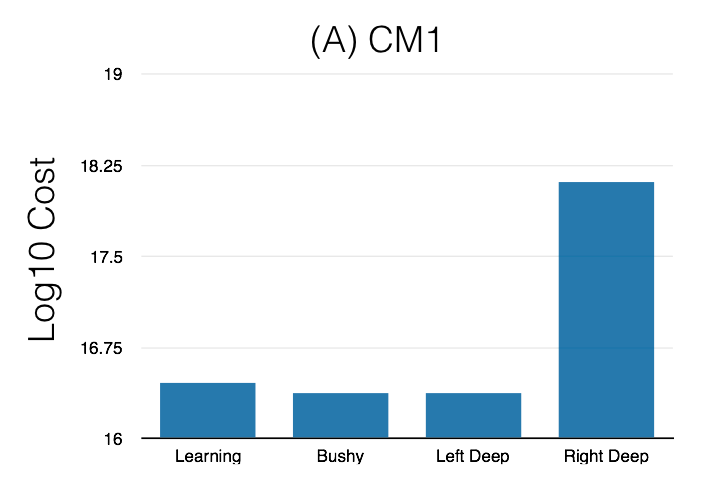
\includegraphics[width=0.24\textwidth]{sql-experiments/1c.png}
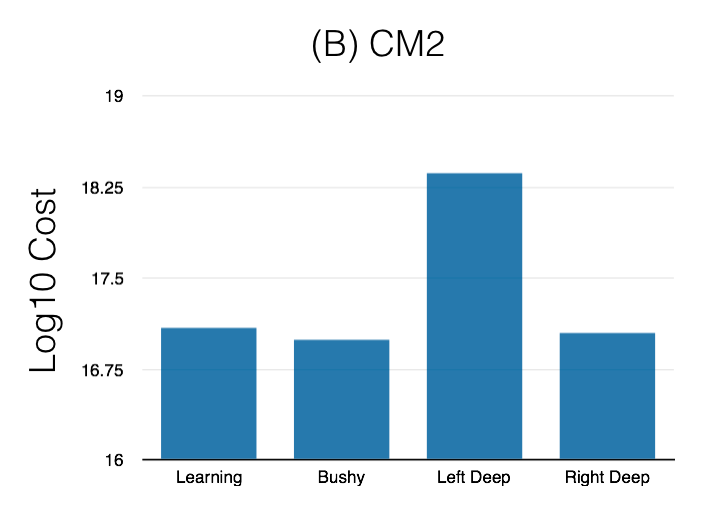
\includegraphics[width=0.24\textwidth]{sql-experiments/1b.png}
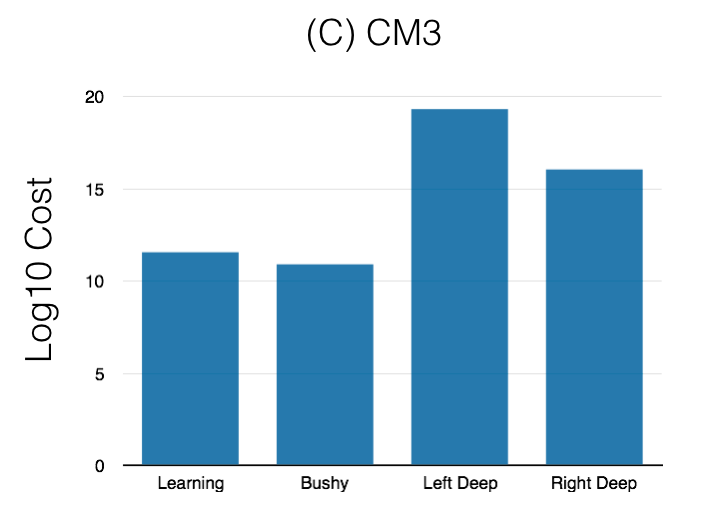
\includegraphics[width=0.24\textwidth]{sql-experiments/1a.png}
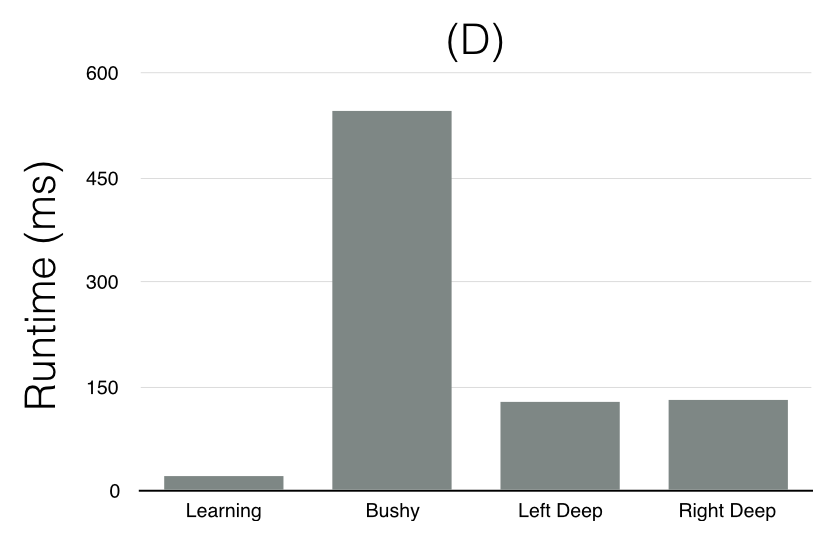
\includegraphics[width=0.24\textwidth]{sql-experiments/1d.png}
\caption{(A) The log cost of the different optimizers with CM1, (B) the log cost of the different optimizers with CM2,  (C) the log cost of the different optimizers with CM3, and (D) the runtime of the different optimizers. \label{sqla}}
\end{figure}


For CM1, we plot the learning curve as a function of the number of training queries (Figure \ref{lcsql}). We actually find that even with 50 training queries, we can consistently find plans competitive with exhaustive search. This suggests that the network is not simply memorizing and is generalizing to unseen subplans.

\begin{figure}[t]
\centering
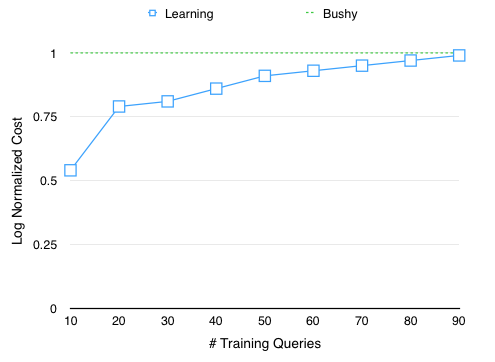
\includegraphics[width=0.5\textwidth]{sql-experiments/2a.png}
\caption{The learning curve as a function of the number of queries. The log normalized cost describes the cost difference between learning and the exhaustive bushy optimizer.  \label{lcsql}}
\end{figure}

\begin{figure}[t]
\centering
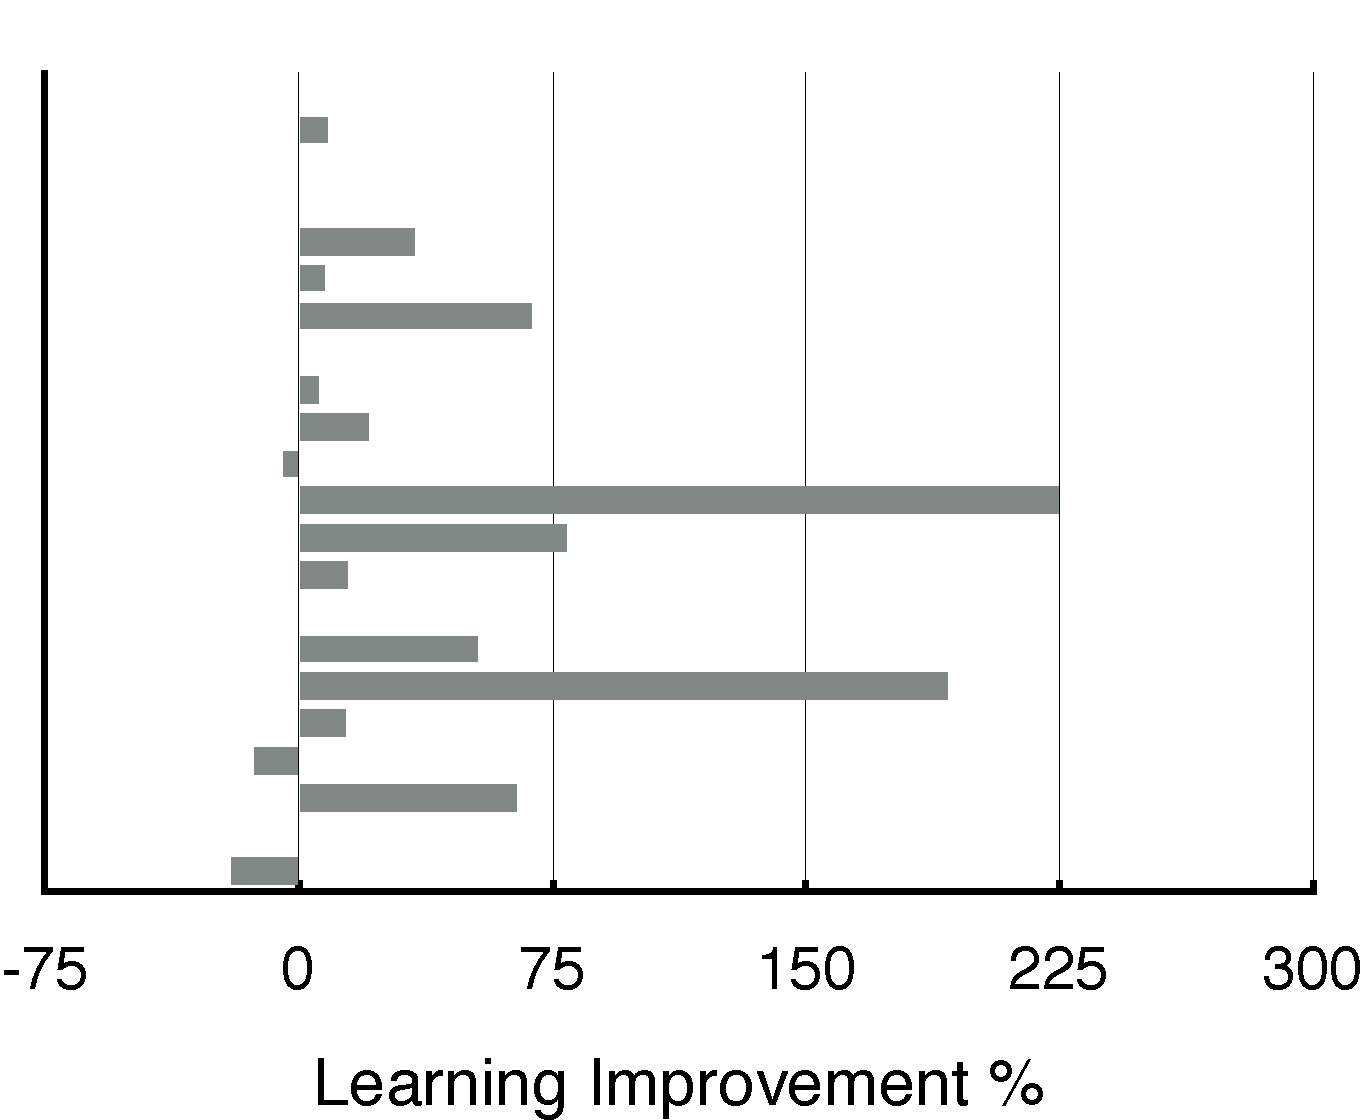
\includegraphics[width=0.4\textwidth]{sql-experiments/tpch.pdf}
\caption{The performance improvement of learning over the postgres query optimizer for each of the TPCH template queries. \label{tpch}}
\end{figure}

\subsection*{TPC-H}
The TPC-H Benchmark is a dataset and workload of SQL queries. It consists of ad-hoc queries and concurrent data modifications. The queries and the data populating the database are inspired by those seen in industry. Unlike the JOB where there is fixed number of queries, TPCH contains a query generator that generates an arbitrary number of queries from templates. In this experiment, we learn the selectivity estimates from data as well.

Using our Apache Calcite connection, we also execute these queries on a real postgres database. Unlike the JOB, these are not idealized cost model. We train the RL algorithm with real runtimes. We first generate 10k training queries for the RL algorithm. Then, we evaluate the RL algorithm on a 100k queries from the generator. We aggregate results by query template. We find that after 10k queries, RL-QUOPT significantly improves on the postgres optimizer on several of the template (Figure \ref{tpch}).

\begin{figure}[t]
\centering
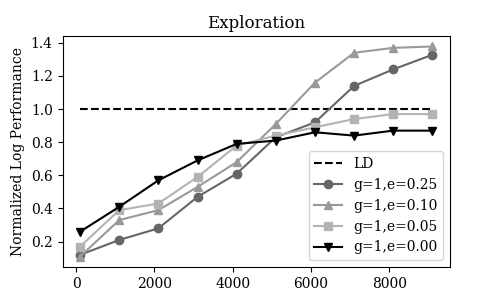
\includegraphics[width=0.32\textwidth]{sql-experiments/exploration-performance.png}
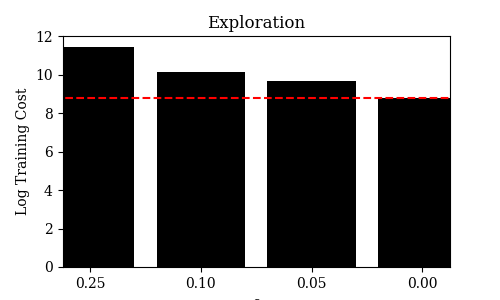
\includegraphics[width=0.32\textwidth]{sql-experiments/exploration2.png}
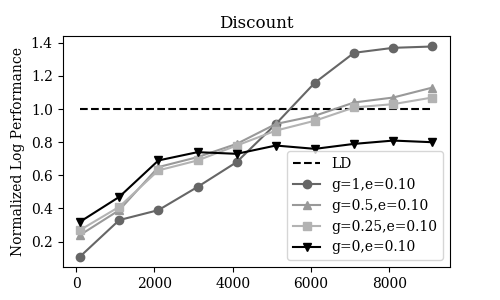
\includegraphics[width=0.32\textwidth]{sql-experiments/discount.png}
\caption{How exploration and discount parameters affect learning performance. \label{exp}}
\end{figure}


The real execution experiment also raises questions about training data collection. During data collection the learner has to execute suboptimal query plans; this could make collecting data very expensive. We evaluate this tradeoff in Figure \ref{exp}. As the exploration parameter $\epsilon$ increases, the query plans executed during training are increasingly suboptimal. However, the learning optimizer has to see a sufficient number of ``bad plans'' to learn an effective optimization policy. Similarly, the discount parameter also affected training performance. Lower discount settings lead to greedier cost attribution--and actually faster training. 


\subsection*{Conclusion}
Reinforcement learning introduces a new approximate dynamic programming framework for SQL query optimization. Classical query optimizers leverage dynamic programs for optimally nesting join queries. This process creates a table that memoizes cost-to-go estimates of intermediate subplans. By representing the memoization table with a neural network, the optimizer can estimate the cost-to-go of even previously unseen plans allowing for a vast expansion of the search space. I show that this process is a form of Deep Q-Learning where the state is a query graph and the actions are contractions on the query graph. One key result is that the same optimization algorithm can adaptively learn search strategies for both in-memory databases (where the search space is often heuristically restricted based to maximize index accesses) and disk-based databases (where the search space is often heuristically restricted to maximize re-use of intermediate results).